%% LyX 2.1.3 created this file.  For more info, see http://www.lyx.org/.
%% Do not edit unless you really know what you are doing.
\documentclass[american]{article}
\usepackage{fontspec}
\usepackage{color}
\usepackage{array}
\usepackage{multirow}
\usepackage{graphicx}
\usepackage[unicode=true,pdfusetitle,
 bookmarks=true,bookmarksnumbered=true,bookmarksopen=true,bookmarksopenlevel=3,
 breaklinks=false,pdfborder={0 0 1},backref=false,colorlinks=true]
 {hyperref}
\hypersetup{
 unicode=false}

\makeatletter

%%%%%%%%%%%%%%%%%%%%%%%%%%%%%% LyX specific LaTeX commands.
%% Because html converters don't know tabularnewline
\providecommand{\tabularnewline}{\\}

%%%%%%%%%%%%%%%%%%%%%%%%%%%%%% User specified LaTeX commands.
\usepackage{indentfirst}
\usepackage{amsmath}
\setlength{\parindent}{2em}

\makeatother

\usepackage{xunicode}
\usepackage{polyglossia}
\setdefaultlanguage[variant=american]{english}
\begin{document}

\title{CASCADE SYSTEM CALCULATION}

\maketitle

\section{Introduction}

Different types of collectors and different technologies for electricity
generation are suitable for different working temperature zones with
different costs. A prototype of cascade collection and cascade utilization
of solar energy with high efficiency and low cost is presented. Parabolic
trough collectors are used to collect low temperature energy with
low cost and dish collectors are used to collect high temperature
energy with high efficiency. Rankine cycle is used to work in low
temperature zone and Stirling cycle is used to work in high temperature
zone. Furthermore, effective topological structures are considered
to take full advantages of thermodynamic characters of different components
of the system. The cold chamber of Stirling engine is cooled by condensed
fluid of Rankine cycle to use the heat released by Stirling engine. 


\section{Problem description}

To characterize the system, calculation of the system must be applied
first. The scale of the system and the dimensions of the parameters
must be evaluated.

Before detailed model of the system can be created, lots of simplifying
assumptions are made:
\begin{itemize}
\item Steady state at nominal load
\item Pressure losses negligible everywhere in the pressure circuit
\item Simplified calculation of processes and equipment
\end{itemize}
\noindent For system 1, water is used as the working fluid of Rankine
cycle. Feed water is used to cool the cold chamber of Stirling engine.
Figure \ref{fig:System-1} shows the sketch of system 1. Air is heated
in the dishes, then used to heat the hot chamber of Stirling engine
and air-water heat exchanger successively. Water is heated in the
cold chamber of Stirling engine, preheater, evaporator, superheater
and air-water heat exchanger successively, and then used to work in
the turbine, cooled in the condenser. Troughs are used to provide
heat for the preheater, evaporator and superheater. Pumps are used
to change the pressure of fluids. State numbers are marked on the
sketch according to its logical position. Numbers with solid circle
means saturated liquid states $(x = 0)$, and with dotted circle means
saturated gas states $(x = 1)$.

\noindent \begin{center}
\begin{figure}
\noindent \centering{}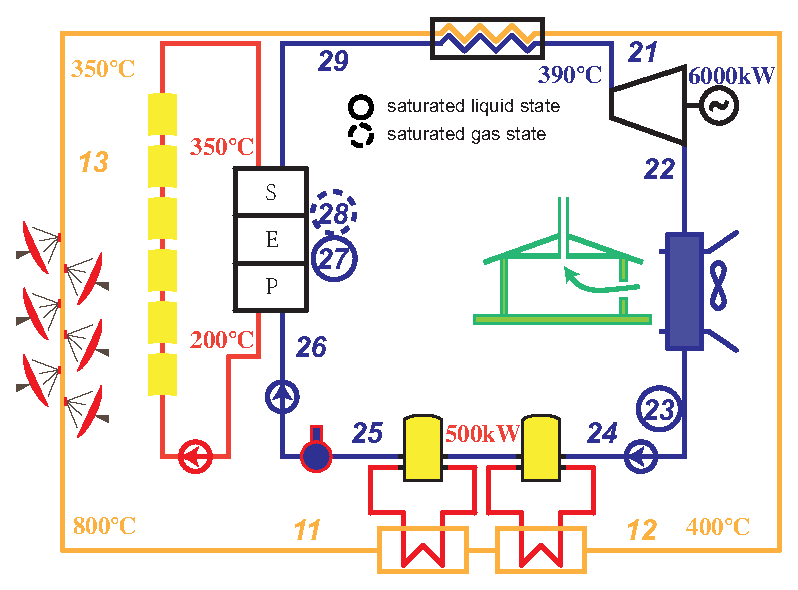
\includegraphics[width=1\textwidth]{System09021}\protect\caption{\label{fig:System-1}Sketch of system 1}
\end{figure}

\par\end{center}


\section{Data}

Table \ref{tab:Table1} shows the basic design data of system 1, such
as the nominal electric power of Stirling engine and generator, temperatures
of inlet and outlet of dishes, design parameters of turbine. According
to these data, some important parameters of the system, such as mass
flow rate, temperature of a state, system efficiency, can be obtained
by calculation. To calculate the system, the model must be built first.
EES is used for the model construction and calculation.

\begin{center}
\begin{table}
\centering{}\protect\caption{\label{tab:Table1}System characteristics of System 1}
\begin{tabular}{|l|l|l|}
\hline 
\multicolumn{3}{|c|}{Nominal electric power}\tabularnewline
\hline 
$P_{stirling} = 500$kWe & $P_{generator} = 6000$kWe & \tabularnewline
\hline 
\multicolumn{3}{|c|}{Solar data}\tabularnewline
\hline 
$DNI = 0.657$kW/m$^2$ &  & \tabularnewline
\hline 
\multicolumn{3}{|c|}{Dish}\tabularnewline
\hline 
$T_{dish,inlet} = 350^{\circ}$C  & $T_{dish,outlet} = 800^{\circ}$C & $p_{dish} = 0.5$MPa\tabularnewline
\hline 
$\eta_{dish} = 0.75$ &  & \tabularnewline
\hline 
\multicolumn{3}{|c|}{Trough}\tabularnewline
\hline 
$T_{trough,inlet} = 200^{\circ}$C  & $T_{trough,outlet} = 350^{\circ}$C  & $p_{trough} = 0.15$MPa\tabularnewline
\hline 
$\eta_{trough} = 0.6$ &  & \tabularnewline
\hline 
\multicolumn{3}{|c|}{Stirling engine}\tabularnewline
\hline 
\multirow{1}{*}{$T_{1,afterstirling} = 400^{\circ}$C} & $T_{environment} = 20^{\circ}$C & $\Delta{}T_{stirling,hot} = 30^{\circ}$C\tabularnewline
\hline 
$\Delta{}T_{stirling,cold} = 25^{\circ}$C & $\eta_{co} = 0.4$ & $p_{2,stirling} = 0.2$MPa\tabularnewline
\hline 
\multicolumn{3}{|c|}{Steam generator}\tabularnewline
\hline 
$T_s = 390^{\circ}$C & $p_s = 2.35$MPa & $p_c = 0.015$MPa\tabularnewline
\hline 
$\dot{m} = 32.09$t/h &  & \tabularnewline
\hline 
\end{tabular}
\end{table}

\par\end{center}


\section{Model of the system}

The system is built in several blocks. These blocks are made of circulations
and efficiency calculation. Two circulations, air circulation and
water circulation, are built in some specific states and in some components.
Known parameters of the states, we can get the efficiency of the system
and the overall efficiency of separated systems.


\subsection{Air circulation}

For State 11,

\begin{equation} 
	\left.\begin{aligned}
		&p_{11} = p_{dish} \\ 
		&T_{11} = T_{dish,outlet} 
	\end{aligned}\right\} \Rightarrow h_{11}
\end{equation}

For state 12, 

\begin{equation} 
	\left.\begin{aligned}
		&p_{12} = p_{11} \\ 
		&T_{12} = T_{1,afterstirling} 
	\end{aligned}\right\} \Rightarrow h_{12}
\end{equation}

For Stirling engine, 

\begin{equation} 
	\begin{aligned}
		&T_{hot} = T_{12} - \Delta{}T_{stirling,hot} \\
		&T_{cold} = T_{25} + \Delta{}T_{stirling,cold} \\
		&\eta_{stirling} = \eta_{co} \cdot (T_{hot} - T_{cold}) / T_{hot}  \\ 
		&Q_{stirling} = P_{stirling} / \eta_{stirling} \\
		&Q_{stirling} = m_1  (h_{11} - h_{12})  \\
		&{\left.\begin{aligned}
			&Q_{stirling,cold} = Q_{stirling} - P_{stirling} \\
			&Q_{stirling,cold} = m_2  (h_{25} - h_{24}) 
		\end{aligned}\right\} \Rightarrow h_{25}}
	\end{aligned}
\end{equation}

For state 13,

\begin{equation}
	\left.\begin{aligned}
		&p_{13} = p_{12} \\
		&T_{13} = T_{dish,inlet}
	\end{aligned}\right\}\Rightarrow h_{13}
\end{equation}

For dish,

\begin{equation}
	\begin{aligned}
		&Q_{dish} = m_1(h_{11} - h_{13}) \\
		&Q_{dish} = DNI \cdot A_{dish} \cdot \eta_{dish}
	\end{aligned}
\end{equation}


\subsection{Water circulation}

For state 21,

\begin{equation}
	\left.\begin{aligned}
		&p_{21} = p_s \\
		&T_{21} = T_s
	\end{aligned}\right\}\Rightarrow
	\left\{\begin{aligned}
		&h_{21} \\
		&s_{21}
	\end{aligned}\right.
\end{equation}

For state 22,

\begin{equation}
	\left.\begin{aligned}
		\left.\begin{aligned}
			&P_{turbine} \\
			&\dot{m}
		\end{aligned}\right\}\Rightarrow 
		h_{22} \\
		p_{22}
	\end{aligned}\right\}\Rightarrow
	\left\{\begin{aligned}
		&T_{22} \\
		&x_{22}
	\end{aligned}\right.
\end{equation}

\begin{equation}
	\left.\begin{aligned}
		\left.\begin{aligned}
			&s_{i,22} = s_{21} \\
			&p_{i,22}
		\end{aligned}\right\}\Rightarrow 
		h_{i,22} \\
		h_{22} 
	\end{aligned}\right\}\Rightarrow 
	\eta_{i,turbine}
\end{equation}

For state 23,

\begin{equation}
	\left.\begin{aligned}
		&p_{23} \\
		&x_{23} = 0
	\end{aligned}\right\}\Rightarrow
	\left\{\begin{aligned}
		&h_{23} \\
		&s_{23} 
	\end{aligned}\right.
\end{equation}

For Rankine cycle,

\begin{equation}
	\begin{aligned}
		&P_{generator} = \eta_{generator}P_{turbine} \\
		&P_{turbine} = m_2(h_{21} - h_{22}) \\
		&\eta_{rankine} = (h_{21} - h_{22}) / (h_{21} - h_{23}) \\
		&\eta_{2, total} = \eta_{rankine}\eta_{generator}
	\end{aligned}
\end{equation}

For state 24,

\begin{equation}
	\left.\begin{aligned}
		&s_{24} = s_{23} \\
		&p_{24} = p_{2,stirling}
	\end{aligned}\right\}\Rightarrow
	\left\{\begin{aligned}
		&T_{24} \\
		&h_{24}
	\end{aligned}\right.
\end{equation}

For state 25,

\begin{equation}
	\left.\begin{aligned}
		&p_{25} = p_{24} \\
		&h_{25}
	\end{aligned}\right\} \Rightarrow
	\left\{\begin{aligned}
		&T_{25} \\
		&s_{25}
	\end{aligned}\right.
\end{equation}

For state 26,

\begin{equation}
	\left.\begin{aligned}
		&p_{26} = p_s \\
		&s_{26} = s_{25}
	\end{aligned}\right\}\Rightarrow
	\left\{\begin{aligned}
		&T_{26} \\
		&h_{26}
	\end{aligned}\right.
\end{equation}

For state 27,

\begin{equation}
	\left.\begin{aligned}
		&p_{27} = p_{26} \\
		&x_{27} = 0
	\end{aligned}\right\}\Rightarrow
	\left\{\begin{aligned}
		&T_{27} \\
		&h_{27}
	\end{aligned}\right.
\end{equation}

For state 28,

\begin{equation}
	\left.\begin{aligned}
		&p_{28} = p_{27} \\
		&x_{28} = 1
	\end{aligned}\right\}\Rightarrow
	\left\{\begin{aligned}
		&T_{28} \\
		&h_{28}
	\end{aligned}\right.
\end{equation}

For air-water heat exchanger,

\begin{equation}
	m_1(h_{12} - h_{13}) = m_2(h_{21} - h_{29}) \Rightarrow h_{29}
\end{equation}

For state 29,

\begin{equation}
	\left.\begin{aligned}
		&p_{29} = p_{28} \\
		&h_{29}
	\end{aligned}\right\}\Rightarrow T_{29}
\end{equation}

For trough,

\begin{equation}
	\begin{aligned}
		&Q_{trough} = m_2(h_{29} - h_{26}) \\
		&Q_{trough} = DNI \cdot A_{trough} \cdot \eta_{trough}
	\end{aligned}
\end{equation}


\subsection{System efficiency calculation}

\begin{equation}
	\begin{aligned}
		&E_{total} = DNI \cdot (A_{dish} + A_{trough}) \\
		&\eta_{system} = (P_{stirling} + P_{generator}) / E_{total} \\
		&T_{cold,separate} = T_{environment} + \Delta{}T_{stirling,cold} \\
		&\eta_{stirling,separate} = \eta_{co} \cdot (T_{hot} - T_{cold,separate}) / T_{hot} \\
		&\eta_{separate} = (Q_{dish}\eta_{stirling,separate} + Q_{trough}\eta_{2,total}) / E_{total}
	\end{aligned}
\end{equation}


\section{Results}

Figure \ref{fig:Main-results} shows main results of the system. From
the results, we can see that the overall of the cascade system $\eta_{system} = 0.1635$
is higher than that of separated system $\eta_{separate} = 0.1581$.
The separated system uses the same collectors of the cascade system
and recirculated cooling water with the same temperature of the environment
is used to cool cold chamber of Stirling engine.

\noindent \begin{center}
\begin{figure}
\noindent \begin{centering}
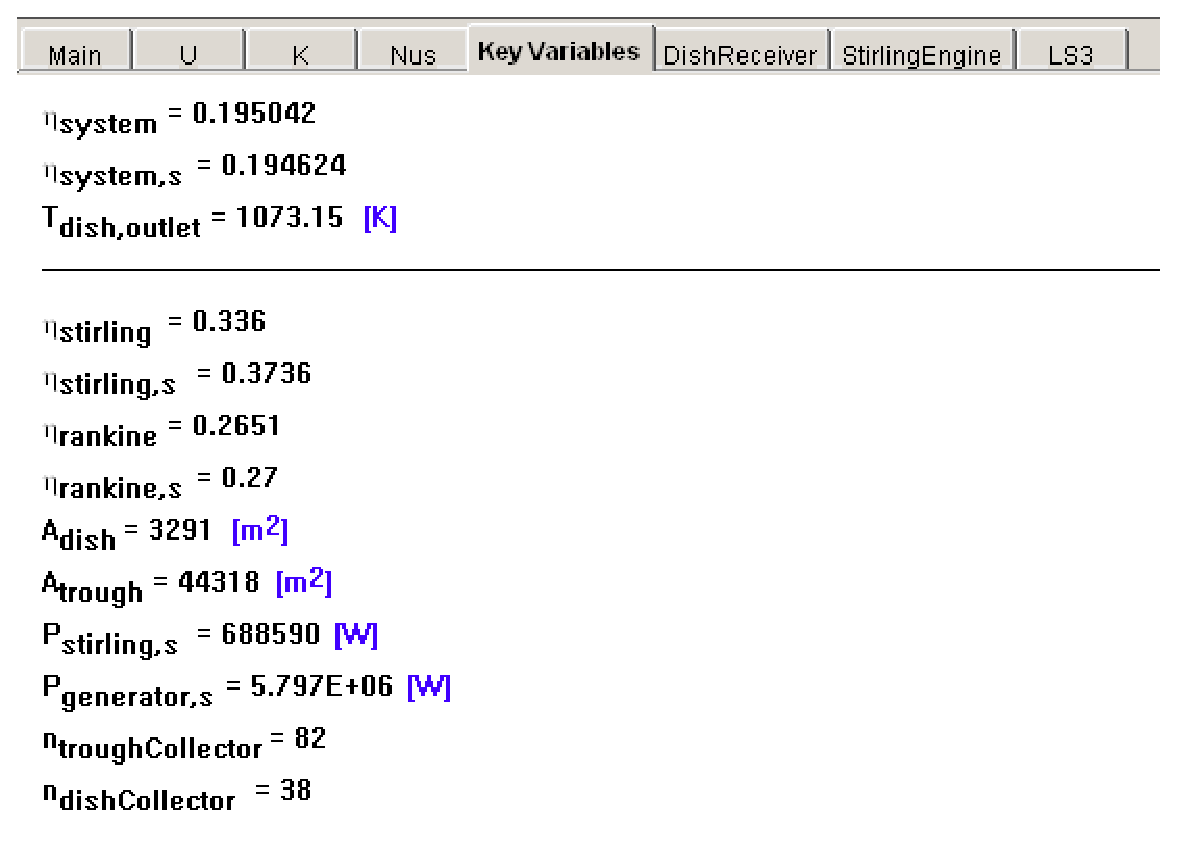
\includegraphics[width=1\textwidth]{System1_results1}\protect\caption{\label{fig:Main-results}Main results}

\par\end{centering}

\end{figure}

\par\end{center}

Figure \ref{fig:Arrays-table-results} shows array table results of
the system. The array shows the enthalpy, pressure, entropy, temperature
and dryness of states. 

\noindent \begin{center}
\begin{figure}
\noindent \begin{centering}
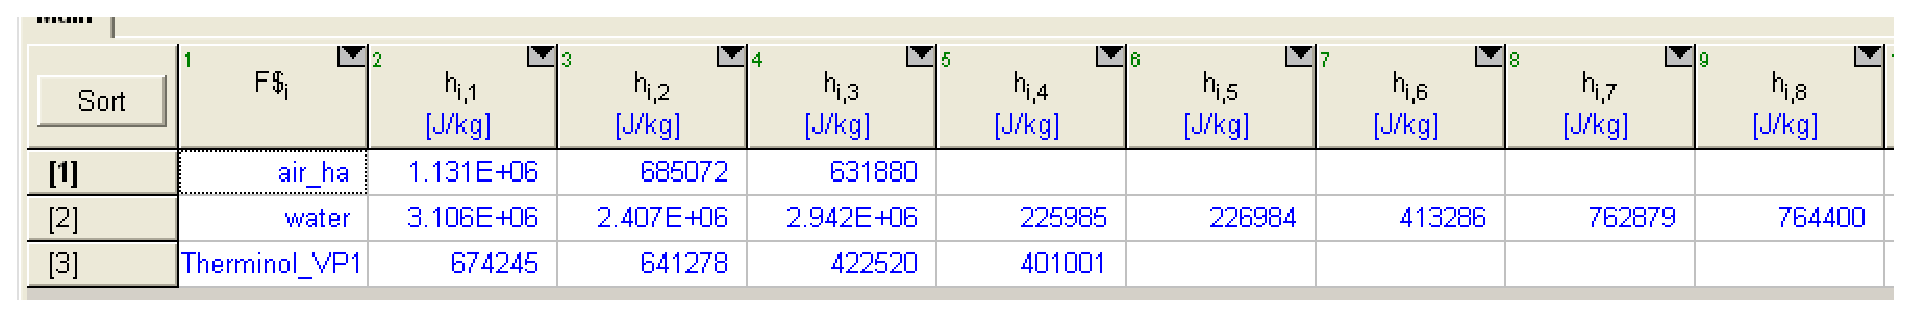
\includegraphics[width=1\textwidth]{System1_results2}\protect\caption{\label{fig:Arrays-table-results}Array table results}

\par\end{centering}

\end{figure}

\par\end{center}
\end{document}
